\subsection*{1. Executar os diferentes servidores em uma máquina diferente da
máquina cliente.}
\addcontentsline{toc}{section}{1. Executar os servidores}

Os \textit{}{Batch Scripts} foram reescritos como \textit{Shell Scripts} com o intuito de serem executados tanto no Linux nativo (Manjaro Linux) quanto no \textit{Windows Subsystem for Linux} (WSL). Os scripts todos estão disponíveis no arquivo zipado, junto com os Batch Scripts


\subsubsection{1.1 - Servidor: executar o rmi.bat e depois o server.bat.}
\addcontentsline{toc}{subsection}{1.1 Execução do servidor}

Primeiramente foi executado o comando rmiregistry, seguido pelo script \texttt{server.sh} para iniciar comunicação com o registro e a armazenação das informações do servidor.

\vspace{2em}
\begin{minipage}{\textwidth}
    \hspace{-1em}
    \centering
    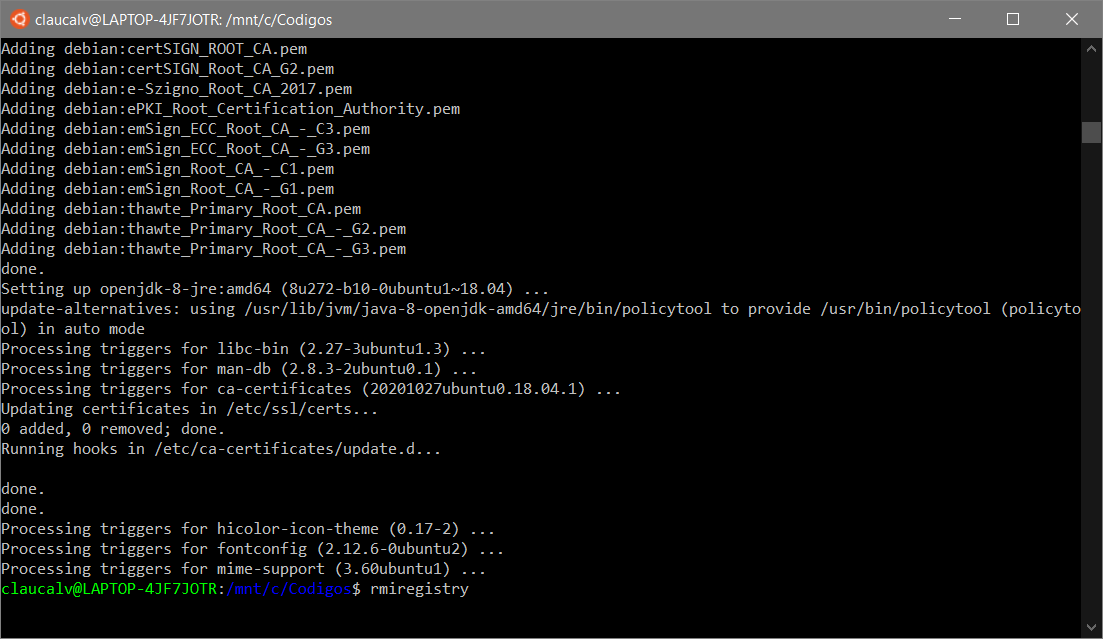
\includegraphics[scale=.35]{prints/rmiregistry.PNG}
    \hspace{1em}
    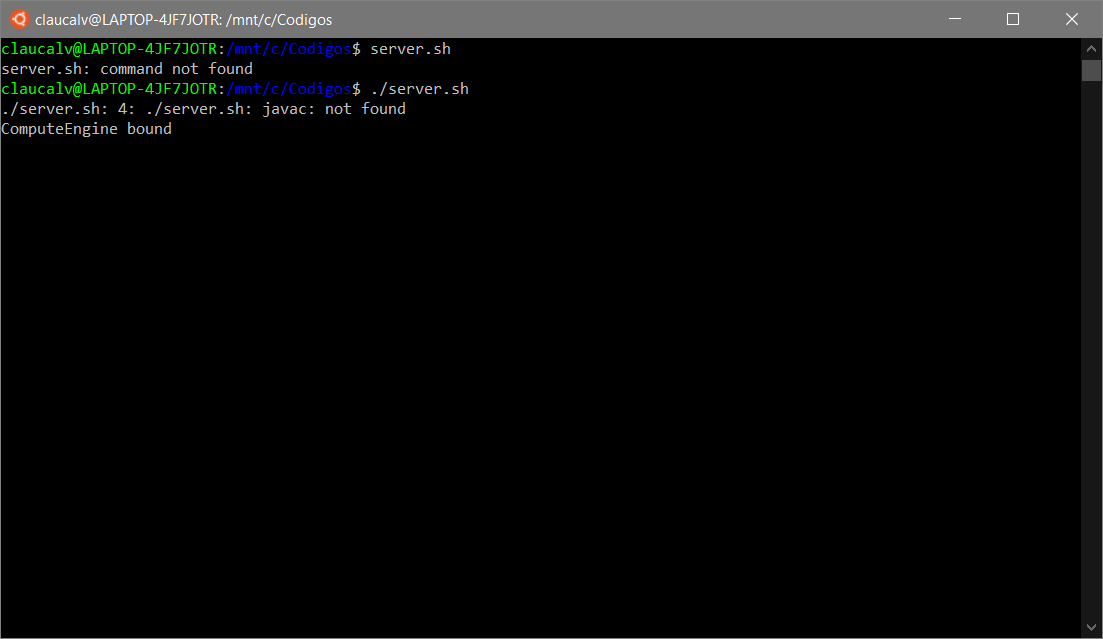
\includegraphics[scale=.35]{prints/server.PNG}
    \captionof{figure}{Execução do rmiregistry e do server}
    \label{threadspng}
    \hspace{1em}
\end{minipage}
\vspace{0.5em}


\subsubsection{1.2 - Cliente: executar o client.bat. Discorra sobre os tempos obtidos na
execução de forma remota e local.}
\addcontentsline{toc}{subsection}{1.2 Execução do client}

Podemos ver todos os sinais de um protocolo TCP, a começar pelo handshake de 3 vias, os pacotes de confirmação entre os pacotes de mensagem, e a finalização bidirecional da comunicação.


\subsection*{2. Executar a classe serialization.SerialObject com os parâmetros adequados (nome de arquivo e operação).}
\addcontentsline{toc}{section}{2. Execução da serialização}

\subsubsection{2.1 - Qual o papel de cada operação (write, read e diff)?}
\addcontentsline{toc}{subsection}{2.1 Diferenças de operação}

\subsection*{3. Implementar um sistema cliente-servidor em que o cliente envia seu objeto Properties a um servidor por meio de socket. O servidor compara o objeto enviado com seu próprio Properties e devolve o resultado da operação diff ao cliente, que é impresso na tela}
\addcontentsline{toc}{section}{3. Implementação cliente-servidor}

